\section{数字信号编码}

\subsection{为什么需要编码}

数字通信系统处理的是0和1组成的序列，但这些二进制数据不能直接在物理信道上传输。原始的二进制流往往包含长串的0或1，这会带来三个问题。

首先，频谱可能不适合信道特性。许多信道（如变压器耦合的线路）无法传输直流分量，而原始二进制流可能有偏（0和1数量不等），导致直流偏移。其次，接收端需要从接收信号中提取时钟以确定抽样时刻。如果流中出现长串连续相同的比特，信号电平长时间不变，定时恢复电路就会失步。第三，原始数据没有内在结构，无法检测传输过程中是否发生错误。

编码的目的，就是将原始二进制序列变换为适合信道传输的波形，同时解决上述三个问题。这不是简单的格式转换，而是在频谱特性、定时信息和检错能力之间的精心权衡。

\begin{figure}[htbp]
    \centering
    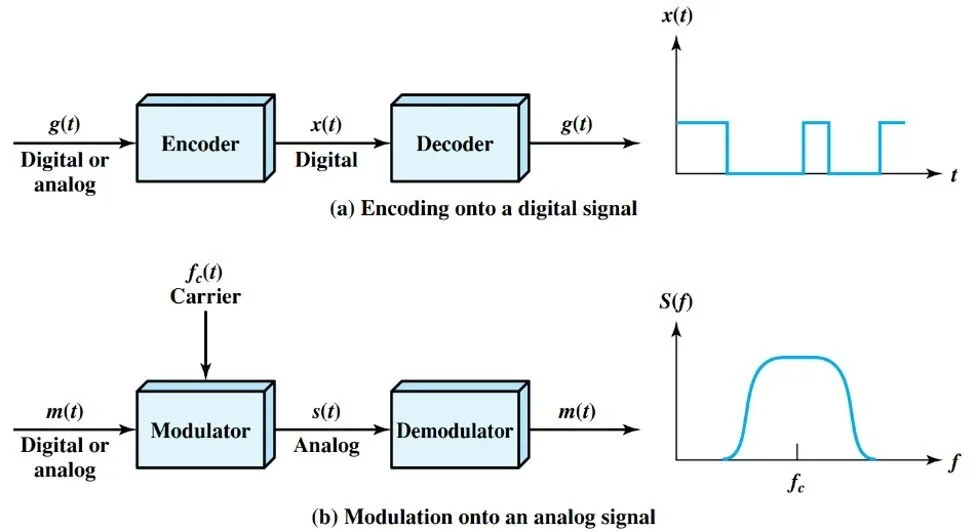
\includegraphics[width=0.9\textwidth]{assets/ch02/ch02-2_4_数字信号编码-000.png}
    \caption{编码与调制的概念对比：(a) 数字信号的编码解码 (b) 模拟信号的调制解调}
    \label{fig:encoding-modulation}
\end{figure}

\subsection{波形的基本属性}

编码首先定义如何用波形表示0和1。单极性波形用正电平和零电平分别表示1和0，实现简单但含有直流分量，不适合交流耦合的远距离传输，仅限于计算机内部或极近距离传输。双极性波形用正电平和负电平分别表示1和0，当0和1等概率出现时无直流分量，更适合远距离传输。

归零与不归零是另一个维度。归零波形的脉冲宽度小于码元周期，在一个码元结束前回到零电平。这种波形的优势在于电平跳变频繁，便于提取定时信息；代价是带宽需求更高。不归零波形占空比100\%，带宽效率更高，但长连0或长连1时没有跳变，定时恢复困难。

曼彻斯特编码是解决定时问题的巧妙方案。每个比特周期中央必有跳变，0用低到高的跳变表示，1用高到低的跳变表示。这样每个比特都自带时钟信息，且正负面积相等，无直流分量。代价是带宽需求加倍，因为最低频率分量对应比特率而非波特率。曼彻斯特编码应用于传统以太网（IEEE 802.3）和RFID系统。

差分编码采用另一种思路。信息编码在相邻码元的电平变化中，而非绝对电平。发生变化表示1，保持不变表示0。这种方式对信道的绝对极性不敏感——即使发送和接收端的正负定义相反，差分编码仍能正确解码。这对于无法确定极性的系统（如某些无线链路）至关重要。

\subsection{线路码的设计原则}

实际传输码型需要在多个目标间权衡。频谱应集中在低频附近，主瓣宽度窄以减少传输带宽，高频分量少以降低对信道带宽的要求，且不含直流以便交流耦合。码流应含有丰富的跳变以支持定时恢复，最好具有内在规律以便检测误码。编译码过程应简单以降低延迟和成本。

没有任何单一码型能完美满足所有要求。AMI码在频谱特性上表现优异，但长连0影响定时；HDB3解决了连零问题，但增加了复杂度；曼彻斯特编码定时性能完美，但带宽效率低下。实际选择取决于具体应用的约束优先级。

\subsection{AMI码：频谱优化的尝试}

传号交替反转码（AMI）的编码规则简洁优雅：0保持为零，1交替变换为正负电平。

以消息序列0110000000110011为例，AMI编码为0 +1 -1 0 0 0 0 0 0 0 -1 +1 0 0 -1 +1。可以看到，正负脉冲交替出现，使直流分量为零。频谱能量集中在频率为1/2码率的附近，高低频分量都很少。

\begin{figure}[htbp]
    \centering
    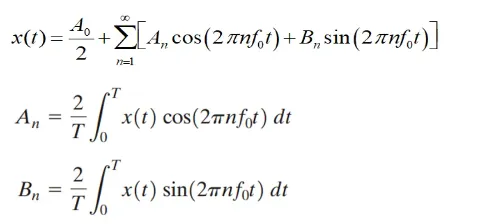
\includegraphics[width=0.8\textwidth]{assets/ch02/ch02-2_4_数字信号编码-003.png}
    \caption{傅里叶级数系数公式：周期信号分解为正弦/余弦波的数学表达}
    \label{fig:fourier-coefficients}
\end{figure}

AMI码还有一个隐藏的优点：可以利用极性交替规律检测误码。正常传输中，正负脉冲应严格交替；如果出现连续两个正脉冲或连续两个负脉冲，必定是传输错误。这为系统提供了宏观的误码监测能力，虽然无法确定具体哪个比特出错，但可以触发告警或维护操作。

但AMI码有一个致命弱点。当原始消息出现长串0时，编码后的波形长时间保持零电平，没有任何跳变。接收端的定时恢复电路依赖跳变来调整本地时钟，长时间无跳变会导致时钟漂移，最终失步。这一缺陷限制了AMI码在高速系统中的应用。

\subsection{HDB3码：解决连零问题}

三阶高密度双极性码（HDB3）是AMI的改进版本，核心思想是将长连0拆散，用特定模式替换，既保持无直流特性，又确保定时信息。

编码规则如下。首先检查消息码中连0的个数，如果连0不超过3个，HDB3与AMI相同。如果连0达到或超过4个，将每4个连0化作一小节，记为B00V，称为破坏节。其中V是破坏脉冲，它的极性与前一个非零脉冲相同——这违反了AMI的交替规则，因此称为"破坏"。B是调节脉冲，取0或正负1，用于保证相邻的V脉冲极性交替。

具体编码过程需要跟踪两个状态：上一个非零脉冲的极性，以及上一个V脉冲的极性。当遇到4个连0时，首先确定V的极性应与前一个非零脉冲相同；然后检查这是否满足"相邻V交替"的规则，如果不满足，则通过设置B来调整。

以消息序列10000100001100000011为例。假设起始极性为负，AMI编码为-1 0 0 0 0 +1 0 0 0 0 -1 +1 0 0 0 0 0 0 0 0 -1 +1。第一组4个连0化作B00V，V应为负（与前一个-1相同）；第二组4个连0，V应为正（与前一个+1相同），且与上一个V（负）交替，满足规则。后续根据同样逻辑继续。最终HDB3编码可能为-1 0 0 0 -V +1 0 0 0 +V -1 +1 -B 0 0 -V +B 0 0 +V -1 +1。

译码过程相对简单。因为每个破坏脉冲V总是与前一个非零脉冲同极性，从接收序列中识别出V的位置，就能确定它前面的三个0和V本身应被还原为4个连0。其余部分按AMI规则译码即可。

HDB3码将连0限制在3个以内，确保了定时信息的提取，同时继承了AMI码无直流、频谱集中的优点。它是我国和欧洲PCM系统的标准码型，A律PCM四次群以下的接口码型均采用HDB3。

\subsection{块编码：另一种思路}

对于更高速率的系统，块编码提供了不同的解决方案。nBmB编码将原始n位二进制码映射为m位二进制码，其中m大于n。在2的m次方种可能组合中，精心选择一部分作为"许用码组"，其余作为"禁用码组"。许用码组的选择标准通常是具有足够频繁的跳变、直流平衡等特性。

以4B5B编码为例。4位信息有16种组合，5位编码有32种组合。从中选择不超过1个前导0和不超过2个后缀0的码组作为许用码组，这样可以保证流中不会出现超过3个连0。如果接收端出现禁用码组，就表明传输过程中发生了错误。

这种编码的代价是带宽增加——5位传输4位信息，效率为80\%。但在光纤等带宽充裕的介质中，这是可以接受的交换。

nBmT编码采用不同策略，将n位二进制码映射为m位三进制码，其中m小于n。例如4B3T编码，4位二进制信息映射为3位三进制符号。由于每位三进制符号可携带$\log_2(3) \approx 1.585$比特信息，3位可携带约4.755比特，大于4比特输入。在相同波特率下，4B3T的信息容量高于二进制编码，提高了频带利用率。这类编码适用于高速同轴电缆传输系统。

\subsection{模数转换的艺术}

模拟信号数字化是数字通信的基石，涉及采样、量化和编码三个步骤。采样将时间连续的信号变为时间离散的样本；量化将幅度连续的样本变为幅度离散的电平；编码将离散电平表示为二进制码。

\subsubsection{采样的理论基础}

奈奎斯特证明了一个基本定理：带宽为B的信号，如果采样率不低于2B，就可以无失真地恢复原信号。这个最低采样率2B称为奈奎斯特率。

定理的物理直觉在于，带宽为B的信号最高频率分量为B，每个周期至少需要采样两次才能确定其振幅和相位。如果采样率低于2B，高频分量会被"混叠"到低频，造成不可恢复的失真。

在实际工程中，采样率通常略高于奈奎斯特率，为信号过渡带和滤波器实现留有余量。例如电话语音带宽约4 kHz，采样率取8 kHz；高保真音频带宽20 kHz，采样率取44.1 kHz或48 kHz。

\subsubsection{量化的权衡}

采样得到的样本幅度仍是连续的，量化将其映射到有限个离散电平。均匀量化将幅度范围等分为若干区间，每个区间对应一个量化电平。这种方法的问题是无论信号电平高低，绝对量化误差相同，导致小信号时的相对误差很大，信噪比恶化。

非均匀量化采用不同策略：小信号区间划分更细，大信号区间划分更粗。这样小信号的量化误差绝对值较小，改善了小信号信噪比；大信号虽然绝对误差较大，但信号本身强，相对误差仍可接受。

非均匀量化通过"压扩"实现。发送端先对信号进行压缩——小信号放大、大信号压缩，然后均匀量化；接收端进行相反的扩张操作。A律和$\mu$律是两种标准的压扩特性，A律主要用于欧洲和中国，$\mu$律用于北美和日本。

\subsubsection{PCM与增量调制}

脉冲编码调制（PCM）是最常用的模数转换方法。以电话系统为例，语音带宽4 kHz，采样率8 kHz，每个样本量化为256级（8比特），得到64 kbps的数据率。这是数字电话系统的标准速率。

增量调制（DM）是另一种思路。它不传输样本的绝对幅度，而是传输相邻样本的变化趋势。在每个采样时刻，比较输入信号与预测值（前一个重建样本）。如果输入大于预测，输出1表示"上升"；如果输入小于预测，输出0表示"下降"。预测值则根据输出更新，上升或下降一个固定步长。

DM实现极为简单，但面临两个挑战。如果信号变化过快，步长跟不上，会产生"斜率过载"失真；如果信号变化缓慢，预测值会在真实值附近震荡，产生"颗粒噪声"。步长的选择是两者的权衡——大步长减少过载但增加颗粒噪声，小步长相反。

相比PCM，DM在相同数据率下信噪比较低，但电路简单、延迟小，适用于对质量要求不高的语音通信或实时控制应用。
